\chapter{Results and Conclusions}

When the algorithms were tested each one was ran ten times. This was to ensure that the results that I was getting were accurate. I did not want to only capture one data point because if I had done this then I could of captured a very good ACO run that gave a short route, this would of not been representative of the overall algorithm. The full result tables are provided in Appendix \ref{apd:result_tables}.

The TSP problems called 100\_node 200\_node and 300\_node were created by me using my TSP file generator. They were modelled after world TSP data. The remaining three TSP files mentioned are VLSI TSP data.

I did make every effort to ensure that my computer was idle when running these tests but some results do stick out as outliers because of either they're much higher or much lower run times. I would like to rerun these tests but due to the high run times of these algorithms I will not be able to do this. 

For the PBM436 TSP I have only managed to run it through once for the ACO only part. I ran out of time to run it the remaining nine times, it took 84474 seconds to run through which is nearly 24 hours. I would have liked to run this through multiple times so that I could be sure that this is an accurate piece of data but in this case it was not possible.

\section{Does clustering allow ACO to be applied to larger problems.}

This question was about seeing if clustering sped up ACO enough for ACO to be applied to larger problems. To see if this was the case I ran six pieces of TSP data: 100\_node, 200\_node, 300\_node, XQF131, XQG237 and PHM436. These are half VLSi data and half self created world data. For each piece of data I ran it using a sole ACO approach and measured the time it took to run, I also ran it using four clustering algorithms: DBSCAN, OPTICS, Affinity Propagation and K-Means. For DBSCAN I used my approach that estimated the eps value and for K-Means I set the node count to 20. Each test was ran ten times and these results are the average of those runs.

It ran with the following ACO parameters: 300 iterations, number of ants is number of nodes divided by 1.5, $\alpha$ is 1, $\beta$ is 10, $\rho$ is 0.4 and $Q$ is 1000.

\begin{longtable}[c]{|p{2cm}|p{1cm}|p{2cm}|p{2cm}|p{3cm}|p{2cm}|}
\hline
\multicolumn{6}{|c|}{The Ratio of Running Speed}                                     \\ \hline
\endhead
%
\multicolumn{6}{|c|}{Ratio = Time(ACO)/Time(Algorithm)}                              \\ \hline
          & ACO   & ACO-DBSCAN & ACO-OPTICS & ACO-AFFINITY-PROPAGATION & ACO-K-MEANS \\ \hline
100\_node & 1.000 & 8.857      & 8.377      & 6.454                    & 11.159      \\ \hline
200\_node & 1.000 & 16.500     & 18.540     & 18.266                   & 32.041      \\ \hline
300\_node & 1.000 & 13.199     & 8.415      & 28.652                   & 39.697      \\ \hline
xqf131    & 1.000 & 7.110      & 3.814      & 13.679                   & 20.944      \\ \hline
xqg237    & 1.000 & 8.437      & 3.317      & 29.225                   & 41.343      \\ \hline
pbm436    & 1.000 & 9.396      & 5.022      & 53.098                   & 58.494      \\ \hline
\caption{This table shows the run time ratios that were achieved. The run time ratio is a measure of how much faster that algorithm is when compared to an ACO only approach, a value of 16.5 means that that particular algorithm is 16.5 times faster than ACO only. This ratio measure was }
\label{tab:run_time_table_question_1}\\
\end{longtable}

Figure \ref{tab:run_time_table_question_1} shows the run time results that were achieved when running these tests.

As the size of the problem increases so too does the improvement gained through the use of clustering, due to the run time of ACO scaling to the square of the number of nodes in the problem it's very important to reduce the number of nodes that ACO runs over in at any particular point. From a run time perspective the best performing algorithms immediately reduce the number of nodes. DBSCAN and OPTICS both have the concept of noise which has the effect of ACO initially running over more nodes. For the 300 node problem DBSCAN generated 21 clusters and 75 nodes and OPTICS generated 20 clusters and 103 nodes, therefore for these two algorithms the run times are a lot higher. Looking at the 300\_node problem even though DBSCAN and OPTICS both have have more nodes for ACO to initially run over they still give massive performance gains.

As the number of nodes increase K\_Means really shows how much it can improve. In the 300\_node problem it generates 20 clusters of roughly equal size, the largest cluster it generates contains 31 nodes. This causes a massive decrease in run time because ACO is running over fewer nodes at any one time.

My results shows that by combining ACO with clustering a considerable run time improvement can be made against a pure ACO approach. This is consistent with what was found in \cite{pang_chao-yang_ben-qiong_zhang_jie_wei_shan_zheng-chao_2014}, here they also showed that ACO can be beaten by clustering algorithms although the clustering algorithms they chose are faster and beat ACO by a higher factor. The only clustering algorithms that we both use is K-Means and our results are very similar for a number of TSPs. They do differ slightly but this can be because of any number of reasons, they don't provide a k value so they may be splitting into more clusters which will slow the process down. They also don't say what type of data these are, there is a link to the data but as of 7th May that link doesn't appear to be working so I can't see how complex or what type of TSP problem they are running.

The clustering algorithms seem to have very different results when running on VLSI problems, OPTICS and DBSCAN both perform very poorly in this situation when compared to 'world' TSP data. It seems like these clustering algorithms are poorly suited to clustering this type of data, the structure of VLSI data performs poorly when clustered with these conventional clustering algorithms. DBSCAN and OPTICS don't manage to place many nodes into clusters it regards most nodes as noise, this has the result that ACO is ran over more nodes which increases the run time. DBSCAN performs better than OPTICS, the automated distance finding for OPTICS is not suited to the patterns presented in VLSI data. I can not make direct comparisons between my runs of VLSI data and the aforementioned paper because I do not know the types of the TSP data that they have used.

K-Means and Affinity Propagation have no problems dealing with VLSI data they are able to cluster it and give very good results.

\section{To what effect do different clustering algorithms have on the quality and run time of the solution.}\label{sec:question2}

This question was about seeing the effect that the clustering algorithm had on ACO, do particular clustering algorithms perform better when combined with ACO to solve a TSP and are they therefore better suited to solve this problem.

To see if there was a clustering algorithm that was better than any others I chose four algorithms: DBSCAN, OPTICS, Affinity Propagation and K-Means. I chose these algorithm because K-Means is similar to Affinity Propagation except that it requires a parameter k, the number of nodes, at the start. DBSCAN and OPTICS are also similar, they both have the concept of noise except OPTICS is designed to be more automated. When I ran DBSCAN I was using my version which found an optimal eps value from the data. 

It ran with the following ACO parameters: 300 iterations, number of ants is number of nodes divided by 1.5, $\alpha$ is 1, $\beta$ is 10, $\rho$ is 0.4 and $Q$ is 1000. The K-Means k value was 20.

\begin{figure}
    \centering
    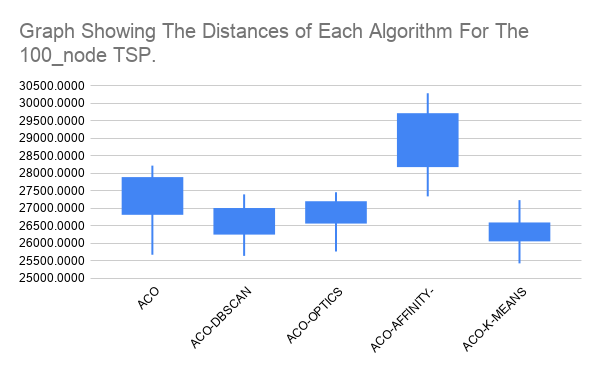
\includegraphics[width=\textwidth]{figures/distance_100_node_graph.png}
    \caption{Box plot showing the distances that were achieved when running the algorithms over the 100\_node TSP. The cut off label reads ACO-Affinity-Propagation.}
    \label{fig:distance_100_node}
\end{figure}

\begin{figure}
    \centering
    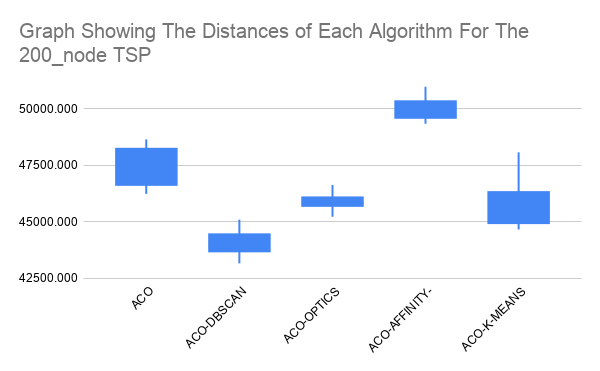
\includegraphics[width=\textwidth]{figures/distance_200_node_graph.png}
    \caption{Box plot showing the distances that were achieved when running the algorithms over the 200\_node TSP. The cut off label reads ACO-Affinity-Propagation.}
    \label{fig:distance_200_node}
\end{figure}

\begin{figure}
    \centering
    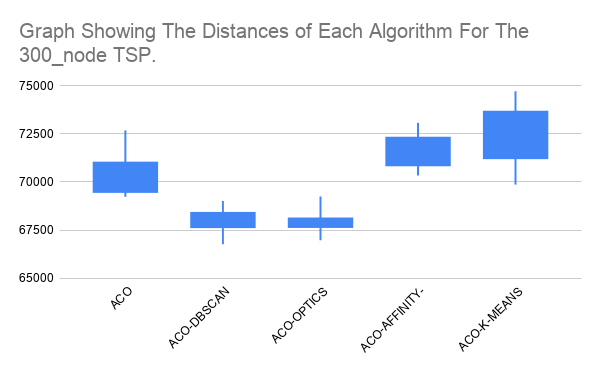
\includegraphics[width=\textwidth]{figures/distance_300_node_graph.png}
    \caption{Box plot showing the distances that were achieved when running the algorithms over the 300\_node TSP. The cut off label reads ACO-Affinity-Propagation.}
    \label{fig:distance_300_node}
\end{figure}

\begin{figure}
    \centering
    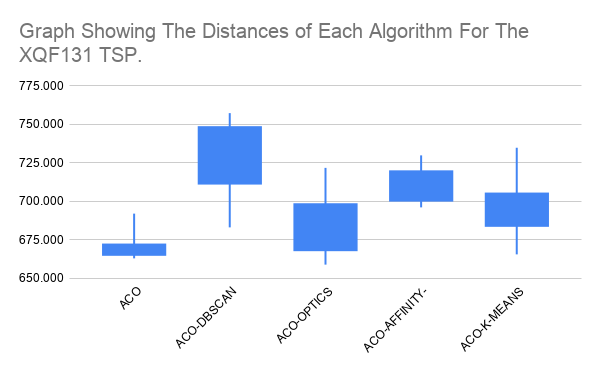
\includegraphics[width=\textwidth]{figures/distance_xqf131_graph.png}
    \caption{Box plot showing the distances that were achieved when running the algorithms over the XQF131 TSP. The cut off label reads ACO-Affinity-Propagation.}
    \label{fig:distance_xqf131}
\end{figure}

\begin{figure}
    \centering
    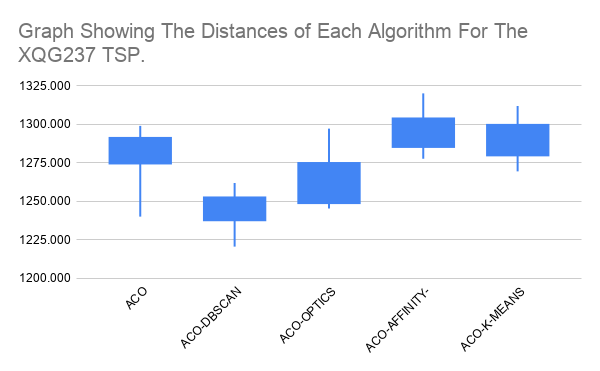
\includegraphics[width=\textwidth]{figures/distance_xqg237_graph.png}
    \caption{Box plot showing the distances that were achieved when running the algorithms over the XQF237 TSP. The cut off label reads ACO-Affinity-Propagation.}
    \label{fig:distance_xqg237}
\end{figure}

\begin{figure}
    \centering
    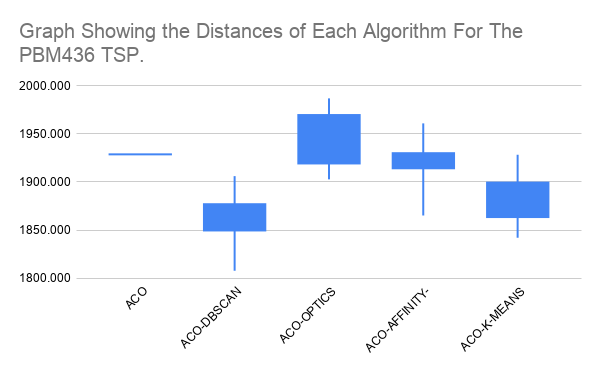
\includegraphics[width=\textwidth]{figures/distance_pbm436_graph.png}
    \caption{Box plot showing the distances that were achieved when running the algorithms over the PBM436 TSP. For this TSP ACO was only ran once due to its incredibly high run time. The cut off label reads ACO-Affinity-Propagation.}
    \label{fig:distance_pbm436}
\end{figure}

Figures \ref{fig:distance_100_node}, \ref{fig:distance_200_node}, \ref{fig:distance_300_node}, \ref{fig:distance_xqf131}, \ref{fig:distance_xqg237} and \ref{fig:distance_pbm436} show the distances that were achieved for these algorithms. These graphs plot the minimum value achieved, the lower quartile, the upper quartile and the maximum value that have been achieved. These quartiles show the spread of the results, the smaller spread would show consistency amongst the results. 

Looking at the world TSP data Affinity Propagation consistently performs worse with poorer results, this could be because it splits the data up into fewer nodes so ACO has less data to work with. Fewer nodes means that it's simpler for ACO to compute the tour but this does mean you don't get the benefits that path finding with ACO provides. Affinity propagation may produce clusters that do not fit the structure of the data very well, it attempts to combine too many nodes into a single cluster which negatively affects the cluster  path finding.

DBSCAN and OPTICS both split the data up into way more nodes than any other algorithm because they support the concept of noise, this leads to ACO initially having more nodes to run over which generates better tours and possibly a better structure which allows the clusters to expand in a way which means the tour is more optimal.

K-Means performs very well especially on the smaller problems it does trail off when the number of nodes are increased though this leads to me thinking that there is an optimal K value depending on the size of the problem, this would be an interesting question to explore. 

For VLSI data all the algorithms seem to be very equal this may be because these algorithm are not really suited to the shapes and complexities of this type of data. The most optimal routes for this types of data follow the paths that the nodes lay out, however the clustering algorithms expand circularly which influences the ACO tour to also follow that pattern. This is why the ACO only tour performs very well on the smaller problem, if it was ran for more iterations then it would of also performed well for the larger problems. For TSP XQG237 ACO can perform very well but is unlikely to and this is down to the number of iterations its more down to luck that it has performed that well.

Optics performs very poorly on this VLSI data, it is unable to find clusters within the data and returns most of the nodes as unclusterable noise. This does mean that it provides tours of reasonable length because ACO is ran over most of the nodes in the problems and isn't bound by any bad clustered structures that OPTICS has returned.

DBSCAN mostly does the best job. It seems to do a good job finding reasonable clusters for this data there is still a lot of unclusterable nodes although less than OPTICS this does lead to better tours being found as well as lower run times. For XQG237 OPTICS finds 15 clusters and 129 unclsuterable nodes, DBSCAN finds 30 clusters and 69 nodes, the clusters that DBSCAN finds map more closely to the patterns in the data. There are a lot more clusters that closely follow the lines presented in the data. Figure \ref{fig:xqg237_optics} and \ref{fig:xqg237_dbscan} shows the clustering that was achieved with DBSCAN and OPTICS and you can see just how much better DBSCAN is, the clusters are smaller and follow the way the data flows. DBSCAN is a lot better at finding clusters with this challenging data.

\begin{figure}
    \centering
    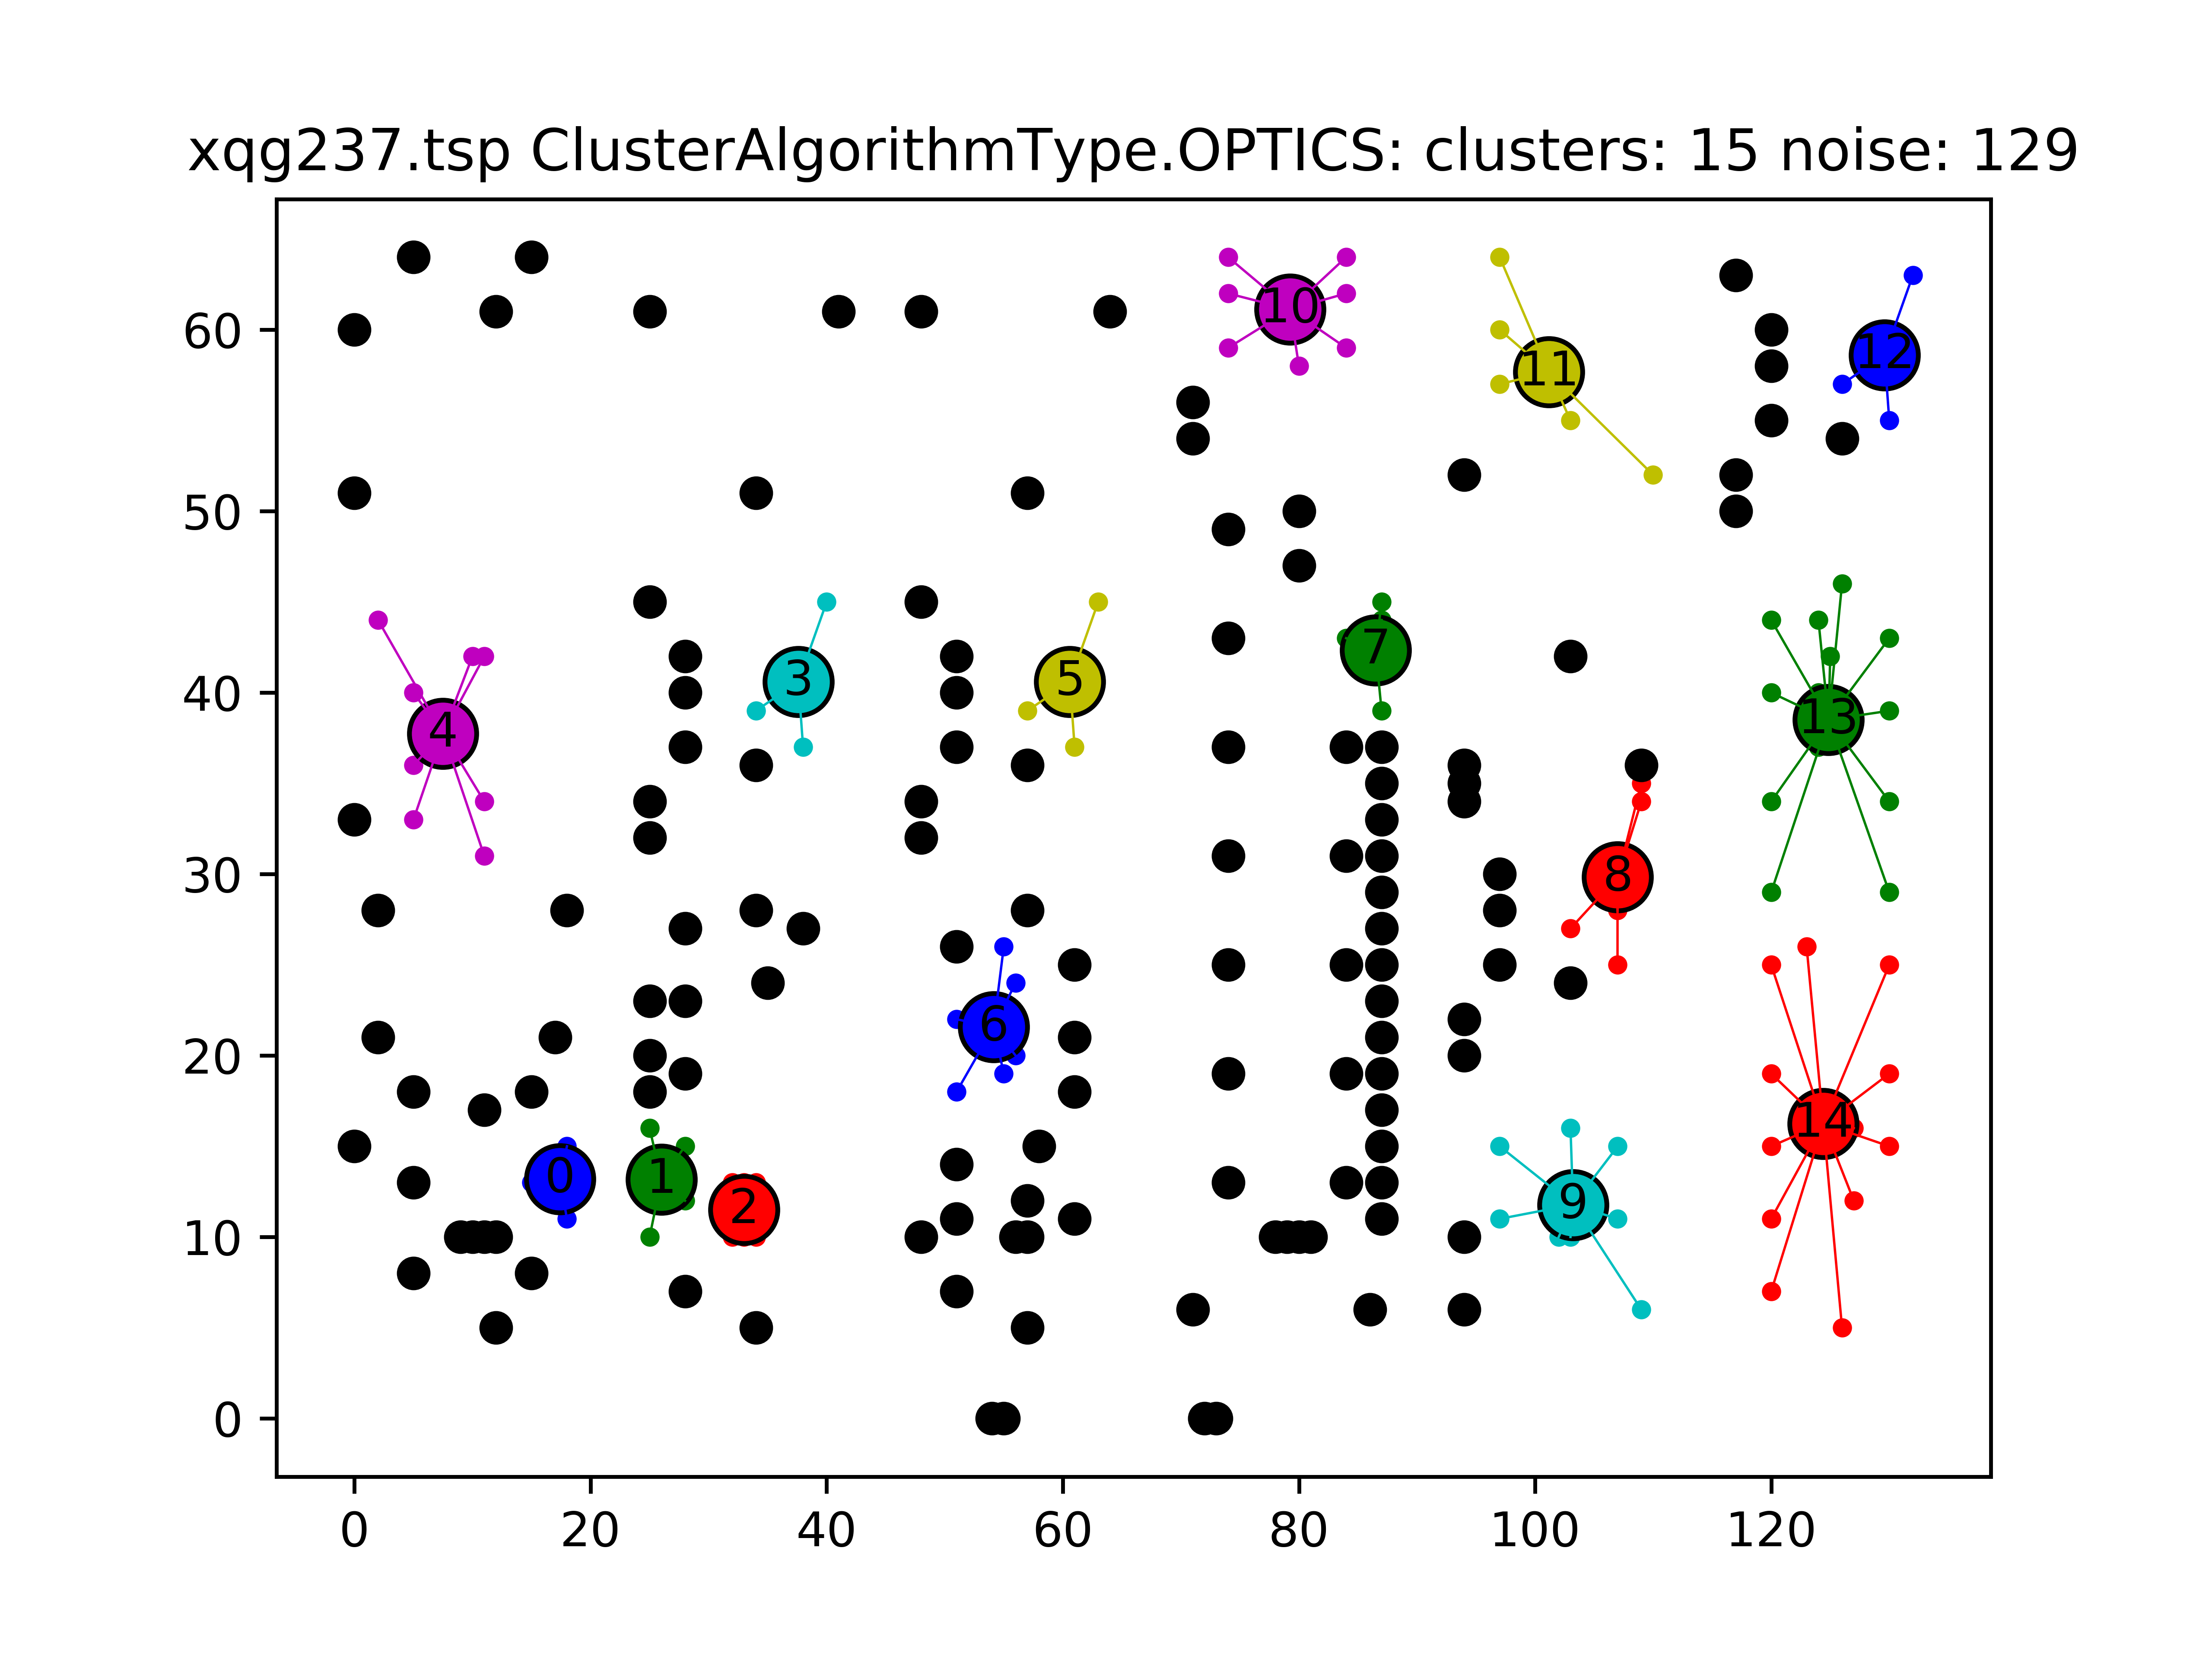
\includegraphics[width=\textwidth]{figures/xqg237_OPTICS.png}
    \caption{The OPTICS clustering for XQG237.}
    \label{fig:xqg237_optics}
\end{figure}

\begin{figure}
    \centering
    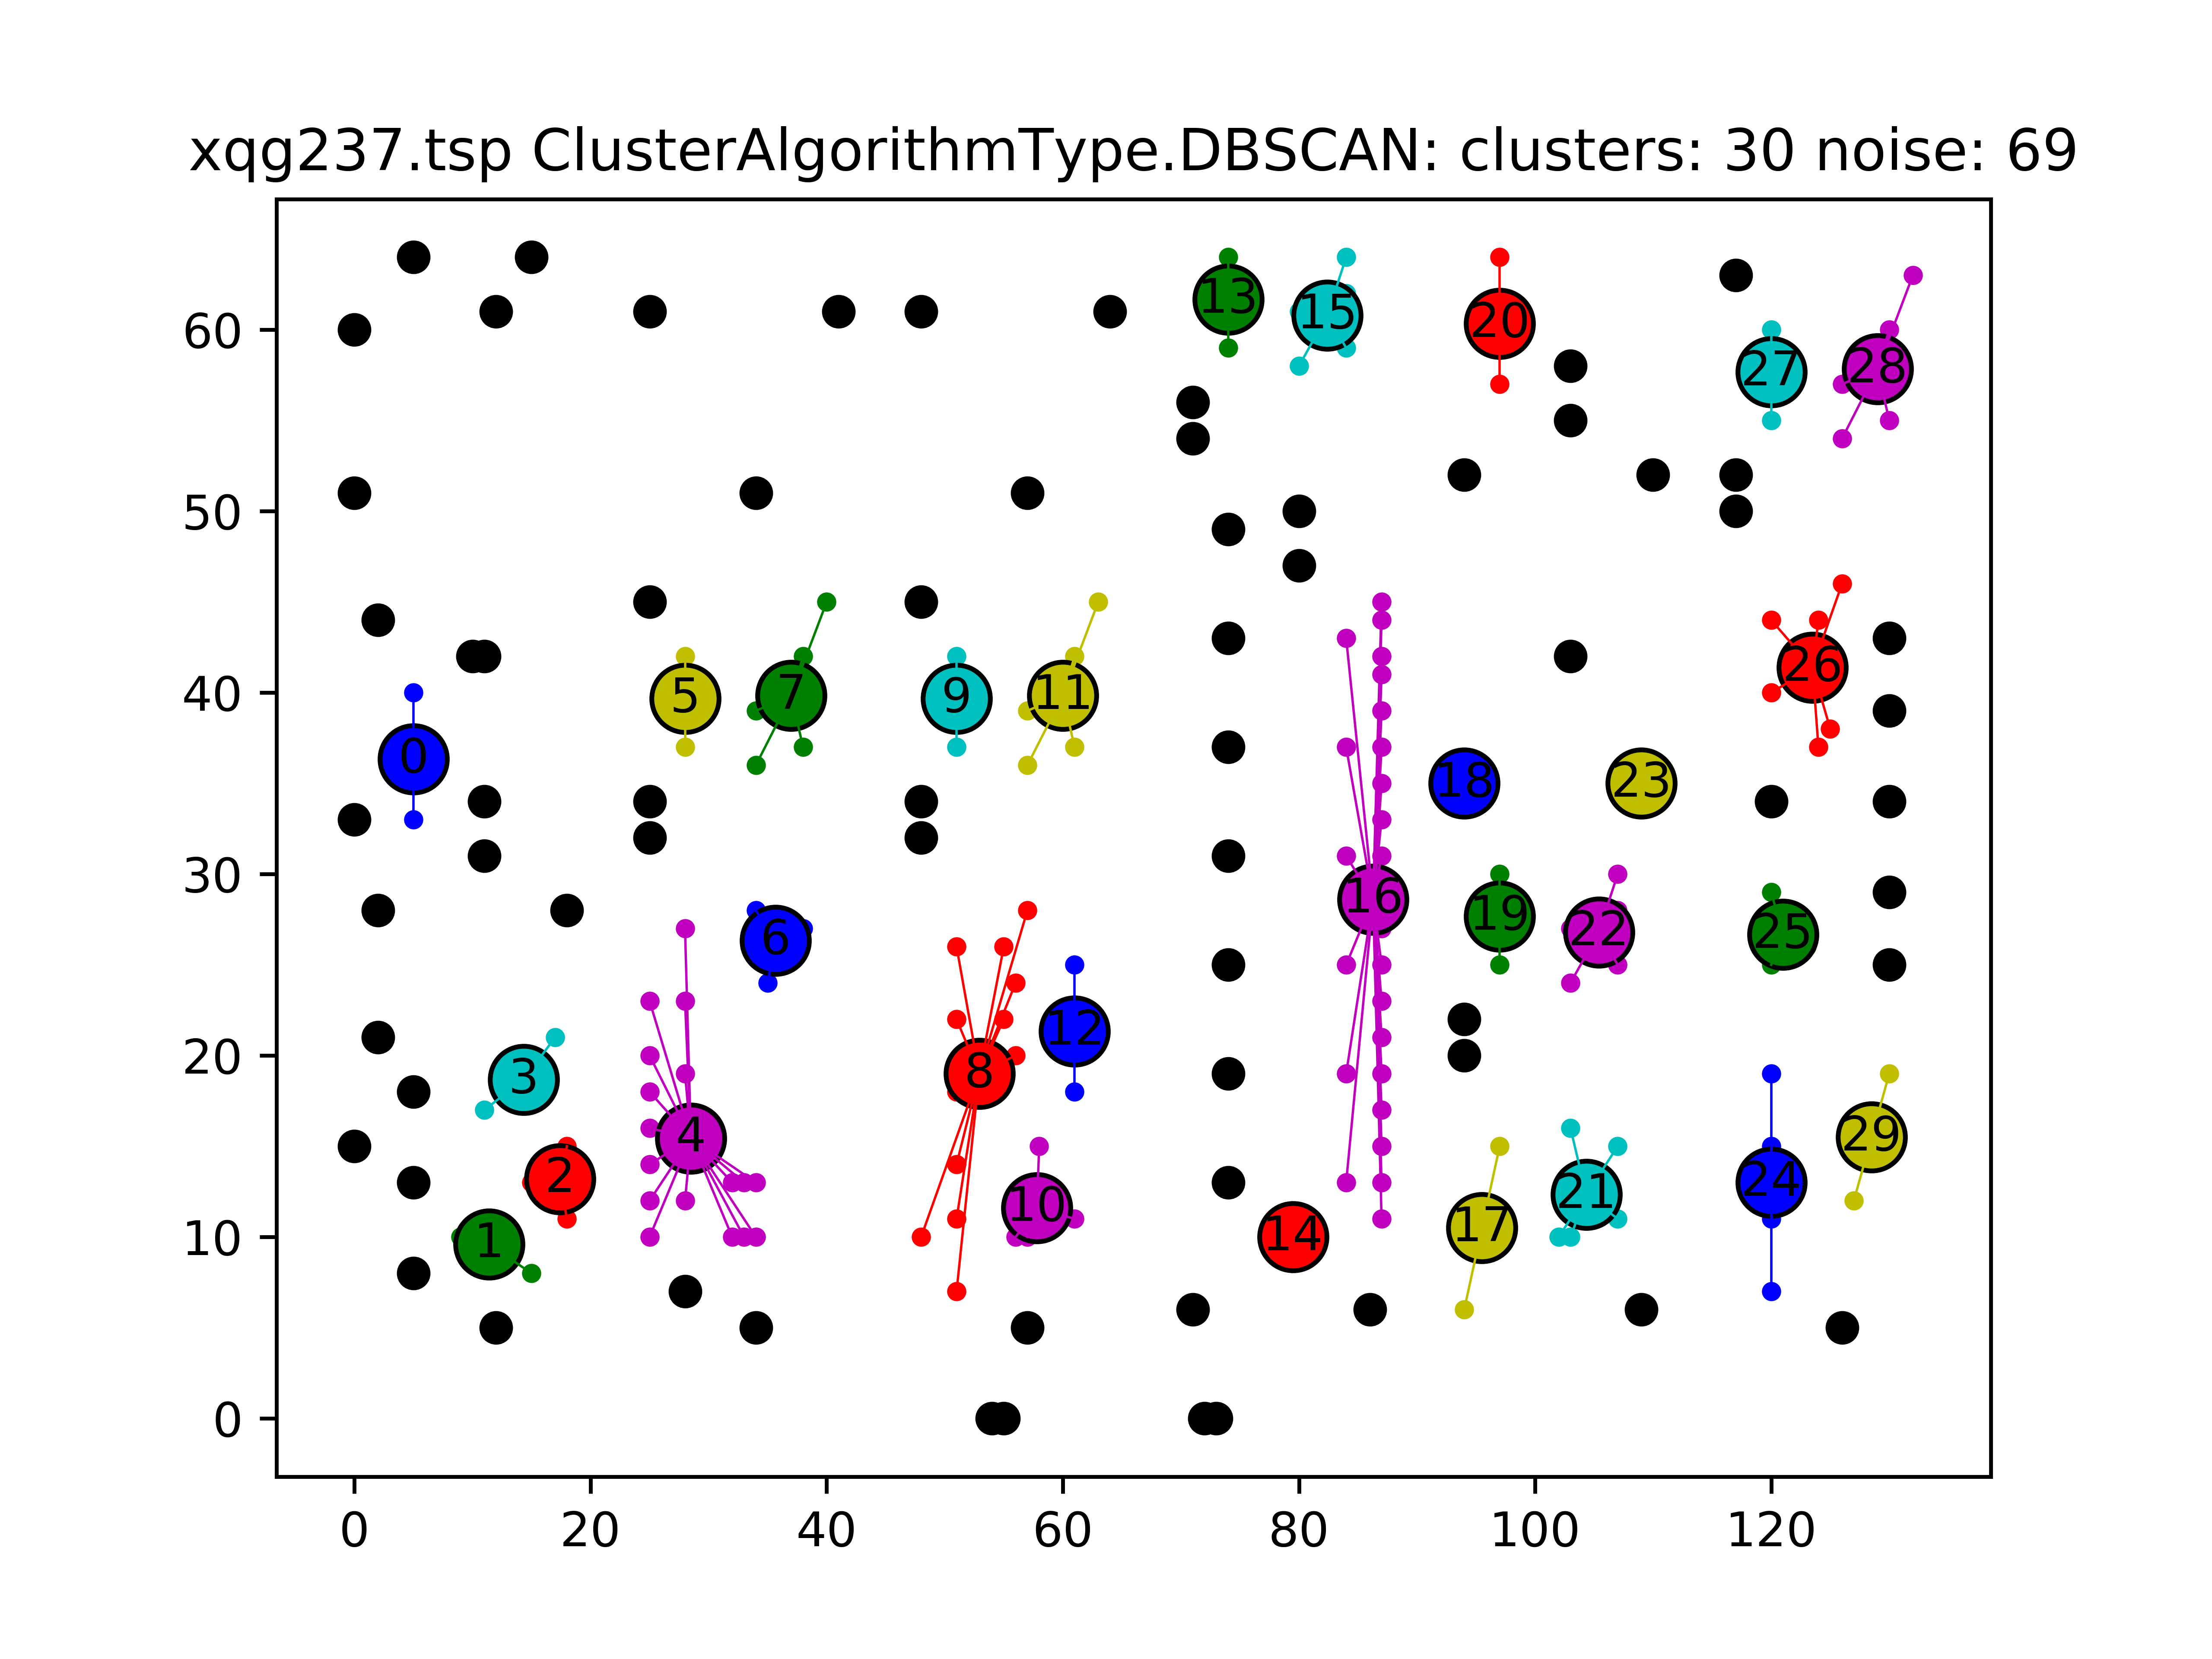
\includegraphics[width=\textwidth]{figures/xqg237_DBSCAN.png}
    \caption{The DBSCAN clustering for XQG237.}
    \label{fig:xqg237_dbscan}
\end{figure}

For VLSI data K-Means performs admirably with a very low run time, it benefits from the many small clusters which greatly reduce the run time of ACO. It doesn't pick out the best patterns in the data as it expands circularly but because a k value of 20 was used there are many clusters and they are all of relatively small sizes.

\begin{longtable}[c]{|p{2cm}|p{1cm}|p{2cm}|p{2cm}|p{3cm}|p{2cm}|}
\hline
\multicolumn{6}{|c|}{The Ratio of Distance To Running Speed}                          \\ \hline
\endhead
%
\multicolumn{6}{|c|}{Ratio = Distance of Algorithm/Run Time of the Algorithm}         \\ \hline
          & ACO    & ACO-DBSCAN & ACO-OPTICS & ACO-AFFINITY-PROPAGATION & ACO-K-MEANS \\ \hline
100\_node & 59.347 & 512.820    & 490.060    & 404.418                  & 640.445     \\ \hline
200\_node & 8.950  & 137.166    & 160.530    & 172.411                  & 276.469     \\ \hline
300\_node & 3.398  & 42.476     & 27.097     & 97.110                   & 135.585     \\ \hline
xqf131    & 0.562  & 4.329      & 2.186      & 8.133                    & 12.229      \\ \hline
xqg237    & 0.131  & 1.080      & 0.430      & 3.895                    & 5.478       \\ \hline
pbm436    & 0.023  & 0.207      & 0.116      & 1.207                    & 1.374       \\ \hline
\caption{This table shows the ratio of distance to run time for each algorithm. It shows how much distance was calculated per second that the algorithm ran for. A higher value does not mean that one algorithm outperformed another it just shows how long it took the algorithm to calculate that length of the tour. A higher value is better. }
\label{tab:ratio_distance_run_time_table}\\
\end{longtable}

From a run time perspective the same factors that I mentioned above are important mainly reducing the number of nodes that ACO runs over at any point. This does lead to K-Means having the best run time out of all the algorithms. Table \ref{tab:ratio_distance_run_time_table} shows a ratio comparing the distance achieved by the algorithm compared to the run time of the algorithm, it represents the distance that was achieved by the algorithm per second, a higher value is better. It shows similar results to what the distance graphs show that the algorithms perform much worse for VLSI data. It also shows how much better K-Means is and how much better it performs compared to the rest.

Overall none of these algorithms can properly deal with the complexities presented in VLSI data, they all expand in a circular fashion which does not work well with that type of data. From a tour length perspective DBSCAN and OPTICS perform better than others but that is mostly because they can not cluster many of the nodes so ACO runs over more nodes increasing the run time and as long as it has ran for sufficient iterations decreases the tour length.


\section{When using 2-opt with ACO and clustering what effect do the clusters have on the overall solution, does 2-opt end up finding the same solution or nearly the same solution regardless of the clustering algorithm used.}

This question was about seeing if the clustering algorithm mattered when you used 2-opt. Did certain clustering algorithms create clusters that were better suited to 2-opt. As the previous experiments have shown the clusters that are produced by the clustering algorithms are very important to the tour that ACO can make. ACO is bound by the tours that are produced in this scenario, but is 2-opt bound by this and if so how much.

To run this experiment I tested six TSPs, three were VLSI and three were World. I used three clustering algorithms for each piece of data OPTICS, DBSCAN and K-Means with a k value of 20. The ACO parameters were: 300 iterations, number of ants is number of nodes divided by 1.5, $\alpha$ is 1, $\beta$ is 10, $\rho$ is 0.4 and $Q$ is 1000. The K-Means k value was 20.

\begin{figure}
    \centering
    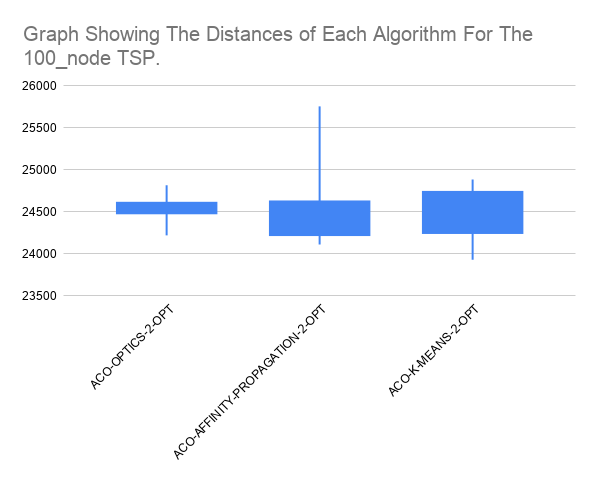
\includegraphics[width=\textwidth]{figures/tsp_distance_100_node_graph.png}
    \caption{Box plot which shows the distances that were achieved when running the algorithms over the 100\_node tsp.}
    \label{fig:tsp_distance_100_node_graph}
\end{figure}

\begin{figure}
    \centering
    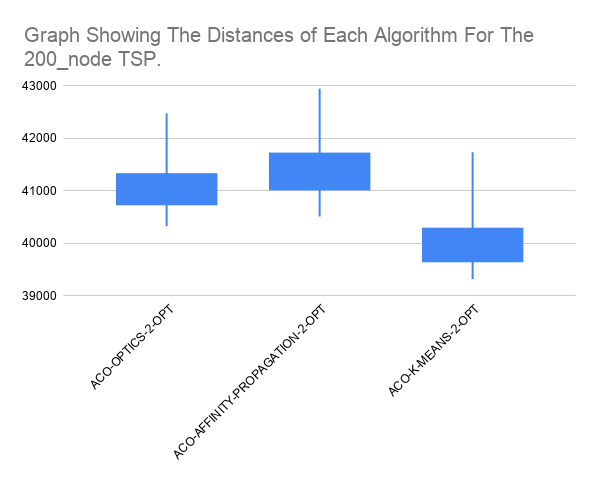
\includegraphics[width=\textwidth]{figures/tsp_distance_200_node_graph.png}
    \caption{Box plot which shows the distances that were achieved when running the algorithms over the 200\_node tsp.}
    \label{fig:tsp_distance_200_node_graph}
\end{figure}

\begin{figure}
    \centering
    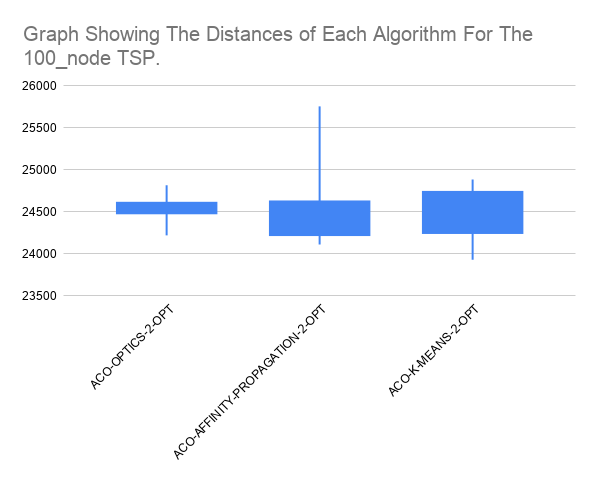
\includegraphics[width=\textwidth]{figures/tsp_distance_100_node_graph.png}
    \caption{Box plot which shows the distances that were achieved when running the algorithms over the 300\_node tsp.}
    \label{fig:tsp_distance_300_node_graph}
\end{figure}

\begin{figure}
    \centering
    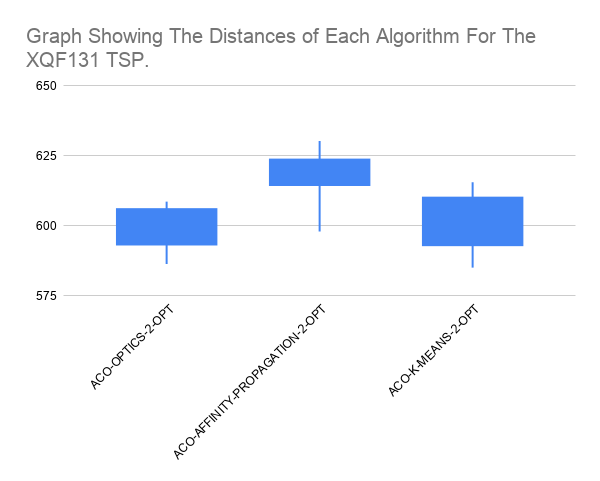
\includegraphics[width=\textwidth]{figures/tsp_distance_xqf131_graph.png}
    \caption{Box plot which shows the distances that were achieved when running the algorithms over the xqf131 tsp.}
    \label{fig:tsp_distance_xqf131_graph}
\end{figure}

\begin{figure}
    \centering
    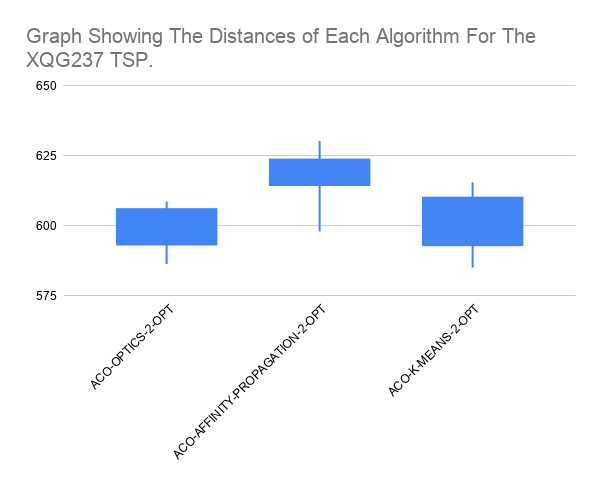
\includegraphics[width=\textwidth]{figures/tsp_distance_xqg237_graph.png}
    \caption{Box plot which shows the distances that were achieved when running the algorithms over the xqg237 tsp.}
    \label{fig:tsp_distance_xqg237_graph}
\end{figure}

\begin{figure}
    \centering
    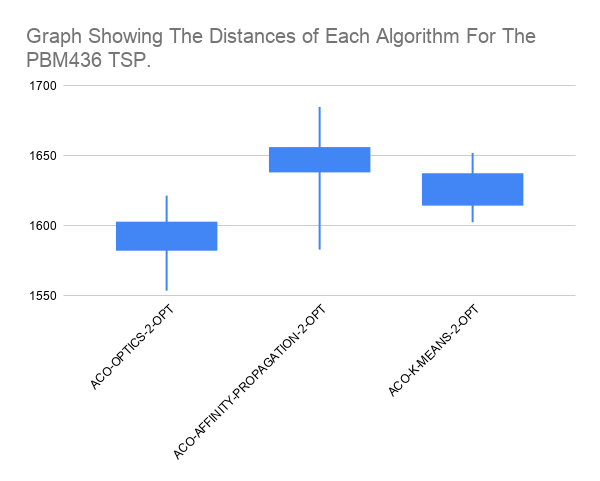
\includegraphics[width=\textwidth]{figures/tsp_distance_pbm436_graph.png}
    \caption{Box plot which shows the distances that were achieved when running the algorithms over the pbm436 tsp.}
    \label{fig:tsp_distance_pbm436_graph}
\end{figure}

Figures \ref{fig:tsp_distance_100_node_graph},  \ref{fig:tsp_distance_200_node_graph},  \ref{fig:tsp_distance_300_node_graph},  \ref{fig:tsp_distance_xqf131_graph},  \ref{fig:tsp_distance_xqg237_graph} and  \ref{fig:tsp_distance_pbm436_graph} show the distances that were achieved for these algorithms.

Comparing these set of graphs to the non 2-opt runs which were presented in section \ref{sec:question2} they show a large improvement. The graphs show a lot less variation and the distances produced are much more consistent amongst the algorithms. 

2-opt is a local search algorithm and therefore will only find the locally optimal solution based on the tour that was passed into it. It is always looking for an improvement and won't make a change to the tour unless it results in a lower tour length, for some tours it will be necessary to make the tour worse in order for an improvement to be found. In order to cut down on the run time it doesn't make these kind of changes. 

The OPTICS run for the 300\_node TSP is interesting because it is much better than the others, the OPTICS run for this problem generates 20 clusters 103 noisy nodes that it can't cluster. This means that the initial ACO run is over 123 nodes, this leads me to believe that structures that the data fall into are very similar amongst all the clustering algorithms and 2-opt finds the optimal version of the tour in this structure. However when you have an algorithm like OPTICS which doesn't put every node into a cluster you end up not falling into that structure and therefore the locally optimal solution that 2-opt finds is different and in this case improved.

VLSI data shows similar results, the tour lengths are closer to each other so the clustering algorithms all return similar clusters that have the same optimal solutions. OPTICS performs better than other algorithms with VLSI data as well, as I've discussed earlier OPTICS performs badly when clustering VLSI data and the same points are true here as well. OPTICS can't cluster the strcutres that are present in VLSI data, it wants to cluster circularly but as VLSI data consists of lines it can't cluster this, and therefore the locally optimal tour that 2-opt finds is the tour that was created by ACO running over lots of nodes.

Affinity Propagation and K-Means give very similar results when 2-opt is ran. The variances of the data are similar as are the average values. It would make sense that these two clustering algorithms give similar results because they work in very similar ways except that Affinity Propagation estimates the number of nodes that are in the data. As both of these algorithms put every node into a cluster it seems that the data and the structure of this data is very similar even though they both produce different amounts of clusters.

These results were not what I was expecting, I assumed that the clusters that were generated would be different enough for the optimal tour that 2-opt found to be significantly different but this turned out to not be the case.

\section{What effect does varying the ACO parameters have on the solution.}

This question was about seeing if there were optimal parameters that could be set on ACO when running with a clustering algorithm. To test this I chose one TSP problem and one clustering algorithm and then varied the parameters to see the effects on both run time and the distance of the tour. When I was testing the parameters I only changed one parameter at a time, the base set of parameters I used was: 300 iterations, number of ants is number of nodes divided by 1.5, $\alpha$ is 1, $\beta$ is 10, $\rho$ is 0.4 and $Q$ is 1000. The K-Means k value was 20. As with all the other experiments I ran this ten times as well. I chose the 200\_node problem to run this on because I thought that it was large enough for the changes to be noticeable but small enough for the runs to not take too long.

I varied the alpha, beta, rho, q and ant count values, for each parameter I tested three values. For alpha I set the values to 0.5, 1 and 1.5, for beta I set the values to 5, 10 and 15, for q I set the values to 500, 1000, 1500, for rho I set the values to 0.2, 0.4 and 1 and I set the ant count to 133, 200 and 400. I chose these values for the ant count because it was the number of nodes in the TSP divided by 1.5, the number of nodes in the TSP and the number of nodes in the TSP multiplied by 2.

\begin{longtable}[c]{|l|l|l|}
\hline
\multicolumn{3}{|c|}{Alpha Value} \\ \hline
\endhead
%
     & Distance     & Run Time    \\ \hline
0.5  & 45609.3870   & 180.5890    \\ \hline
1    & 45733.7063   & 165.4209   \\ \hline
1.5  & 46122.7783  & 180.5890 \\ \hline
\caption{This table shows the average run times and tour lengths when the alpha values where varied.}
\label{tab:alpha_aco_table}\\
\end{longtable}

\begin{longtable}[c]{|l|l|l|}
\hline
\multicolumn{3}{|c|}{Ant Count}  \\ \hline
\endfirsthead
%
\endhead
%
    & Distance    & Run Time   \\ \hline
133 & 45733.7063 & 165.4208  \\ \hline
200 & 45398.0928 & 223.1873 \\ \hline
400 & 45441.4907 & 431.1539 \\ \hline
\caption{This table shows the run times and tour lengths when the ACO ant count werre varied. Here the number of ants was varied so that it was the number of nodes/1.5, the number of nodes and the number of nodes * 2.}
\label{tab:ant_count_aco_table}\\
\end{longtable}

\begin{longtable}[c]{|l|l|l|}
\hline
\multicolumn{3}{|c|}{Beta}     \\ \hline
\endfirsthead
%
\endhead
%
   & Distance    & Run Time  \\ \hline
5  & 45505.8459 & 177.9760   \\ \hline
10 & 45733.7063 & 165.4209   \\ \hline
15 & 45788.4176 & 154.8633 \\ \hline
\caption{This table shows the the run time and tour length when varying the beta value.}
\label{tab:beta_aco_table}\\
\end{longtable}

\begin{longtable}[c]{|l|l|l|}
\hline
\multicolumn{3}{|c|}{Q}      \\ \hline
\endfirsthead
%
\endhead
%
     & Distance   & Run Time \\ \hline
500  & 45505.8459 & 177.9760 \\ \hline
1000 & 45733.7063 & 165.4209 \\ \hline
1500 & 45788.4176 & 154.8633 \\ \hline
\caption{This table shows the run times and tour lengths when varying the Q ACO parameter.}
\label{tab:q_aco_table}\\
\end{longtable}

\begin{longtable}[c]{|l|l|l|}
\hline
\multicolumn{3}{|c|}{Rho}    \\ \hline
\endfirsthead
%
\endhead
%
     & Distance   & Run Time \\ \hline
500  & 45505.8459 & 177.9760 \\ \hline
1000 & 45733.7063 & 165.4209 \\ \hline
1500 & 45788.4176 & 154.8633 \\ \hline
\caption{This table shows the run times and lengths when varying the rho ACO parameter.}
\label{tab:rho_aco_table}\\
\end{longtable}

Tables \ref{tab:ant_count_aco_table}, \ref{tab:q_aco_table}, \ref{tab:rho_aco_table}, \ref{tab:beta_aco_table} and \ref{tab:alpha_aco_table} show the results of varying these parameters. 

These results don't show a huge difference the tour lengths are very similar amongst all the parameters. There are a few differences that can be mentioned. The lower Q value improves the length of the tour, Q affects how much pheromone gets deposited. This means that the ants are more likely to choose a new path because the scent isn't as strong. This could just be random chance though because even though I've ran this ten times ACO still has elements of randomness so these could just be good runs and the ants have randomly chosen good pathways.

Increasing the number of ants increases the run time quite a lot, this does make sense though because the more ants there are to simulate the more times the algorithm has to run so the longer it will take. As shown in Chapter 1 the run time of ACO is proportional to the number of ants.

This question might of not been broad enough and not run the right sets of parameters. Instead of changing one parameter it might of been better to change many parameters at one time, in \cite{gaertner_clark} they attempted to find the optimal ACO parameters and changed three parameters: beta, rho and \[q_{0}\]. They varied each of these parameters and ran the test ten times for each combination this resulted in 13,860 runs. This did get them a result though and they did identify optimal values, this is a question that could be explored further in the future. 